\documentclass[24pt]{article}%book, report,ctexart,ctexreport

%导言区



\usepackage{graphicx}
\usepackage{color}
\usepackage{underscore}

\usepackage[table ]{ xcolor}

\title{
\includegraphics[width=20mm, height=24mm]{SAR.jpg}\\
\textbf \textrm {Team information for L.W.R.A}}
 
\author{Lishaogang Wangyuan Raunhengyu Aimee}
\date{\today}

\newcommand{\tabincell}[2]{\begin{tabular}{@{}#1@{}}#2\end{tabular}}
%正文区,有且只能有一个document
\begin{document}
	
	\maketitle
	
	\renewcommand\arraystretch{1.5}
	
	
	
	\begin{table}[h]
		\begin{center}  
			\begin{tabular}{| p{2cm} | c | c | c | c |}  \hline
	            \rowcolor{lightgray} \multicolumn{5}{c|}{ L.W.R.A } \\ \hline
	            
				\color{blue}\textbf \textrm{Team Member} & Lishaogang & Wangyuan & Raunhengyu & Aimee \\ \hline
				
				\color{blue}\textbf \textrm \tabincell{c}{Email} & \tabincell{c}{gravitation2358\\@gmail.com} & \tabincell{c}{963671029\\@qq.com} & \tabincell{c}{hengyudd\\@gmail.com} & \tabincell{c}{aimee_yanjc\\@163.com}\\ \hline
				
				\color{blue}\textbf \textrm{Photo} & 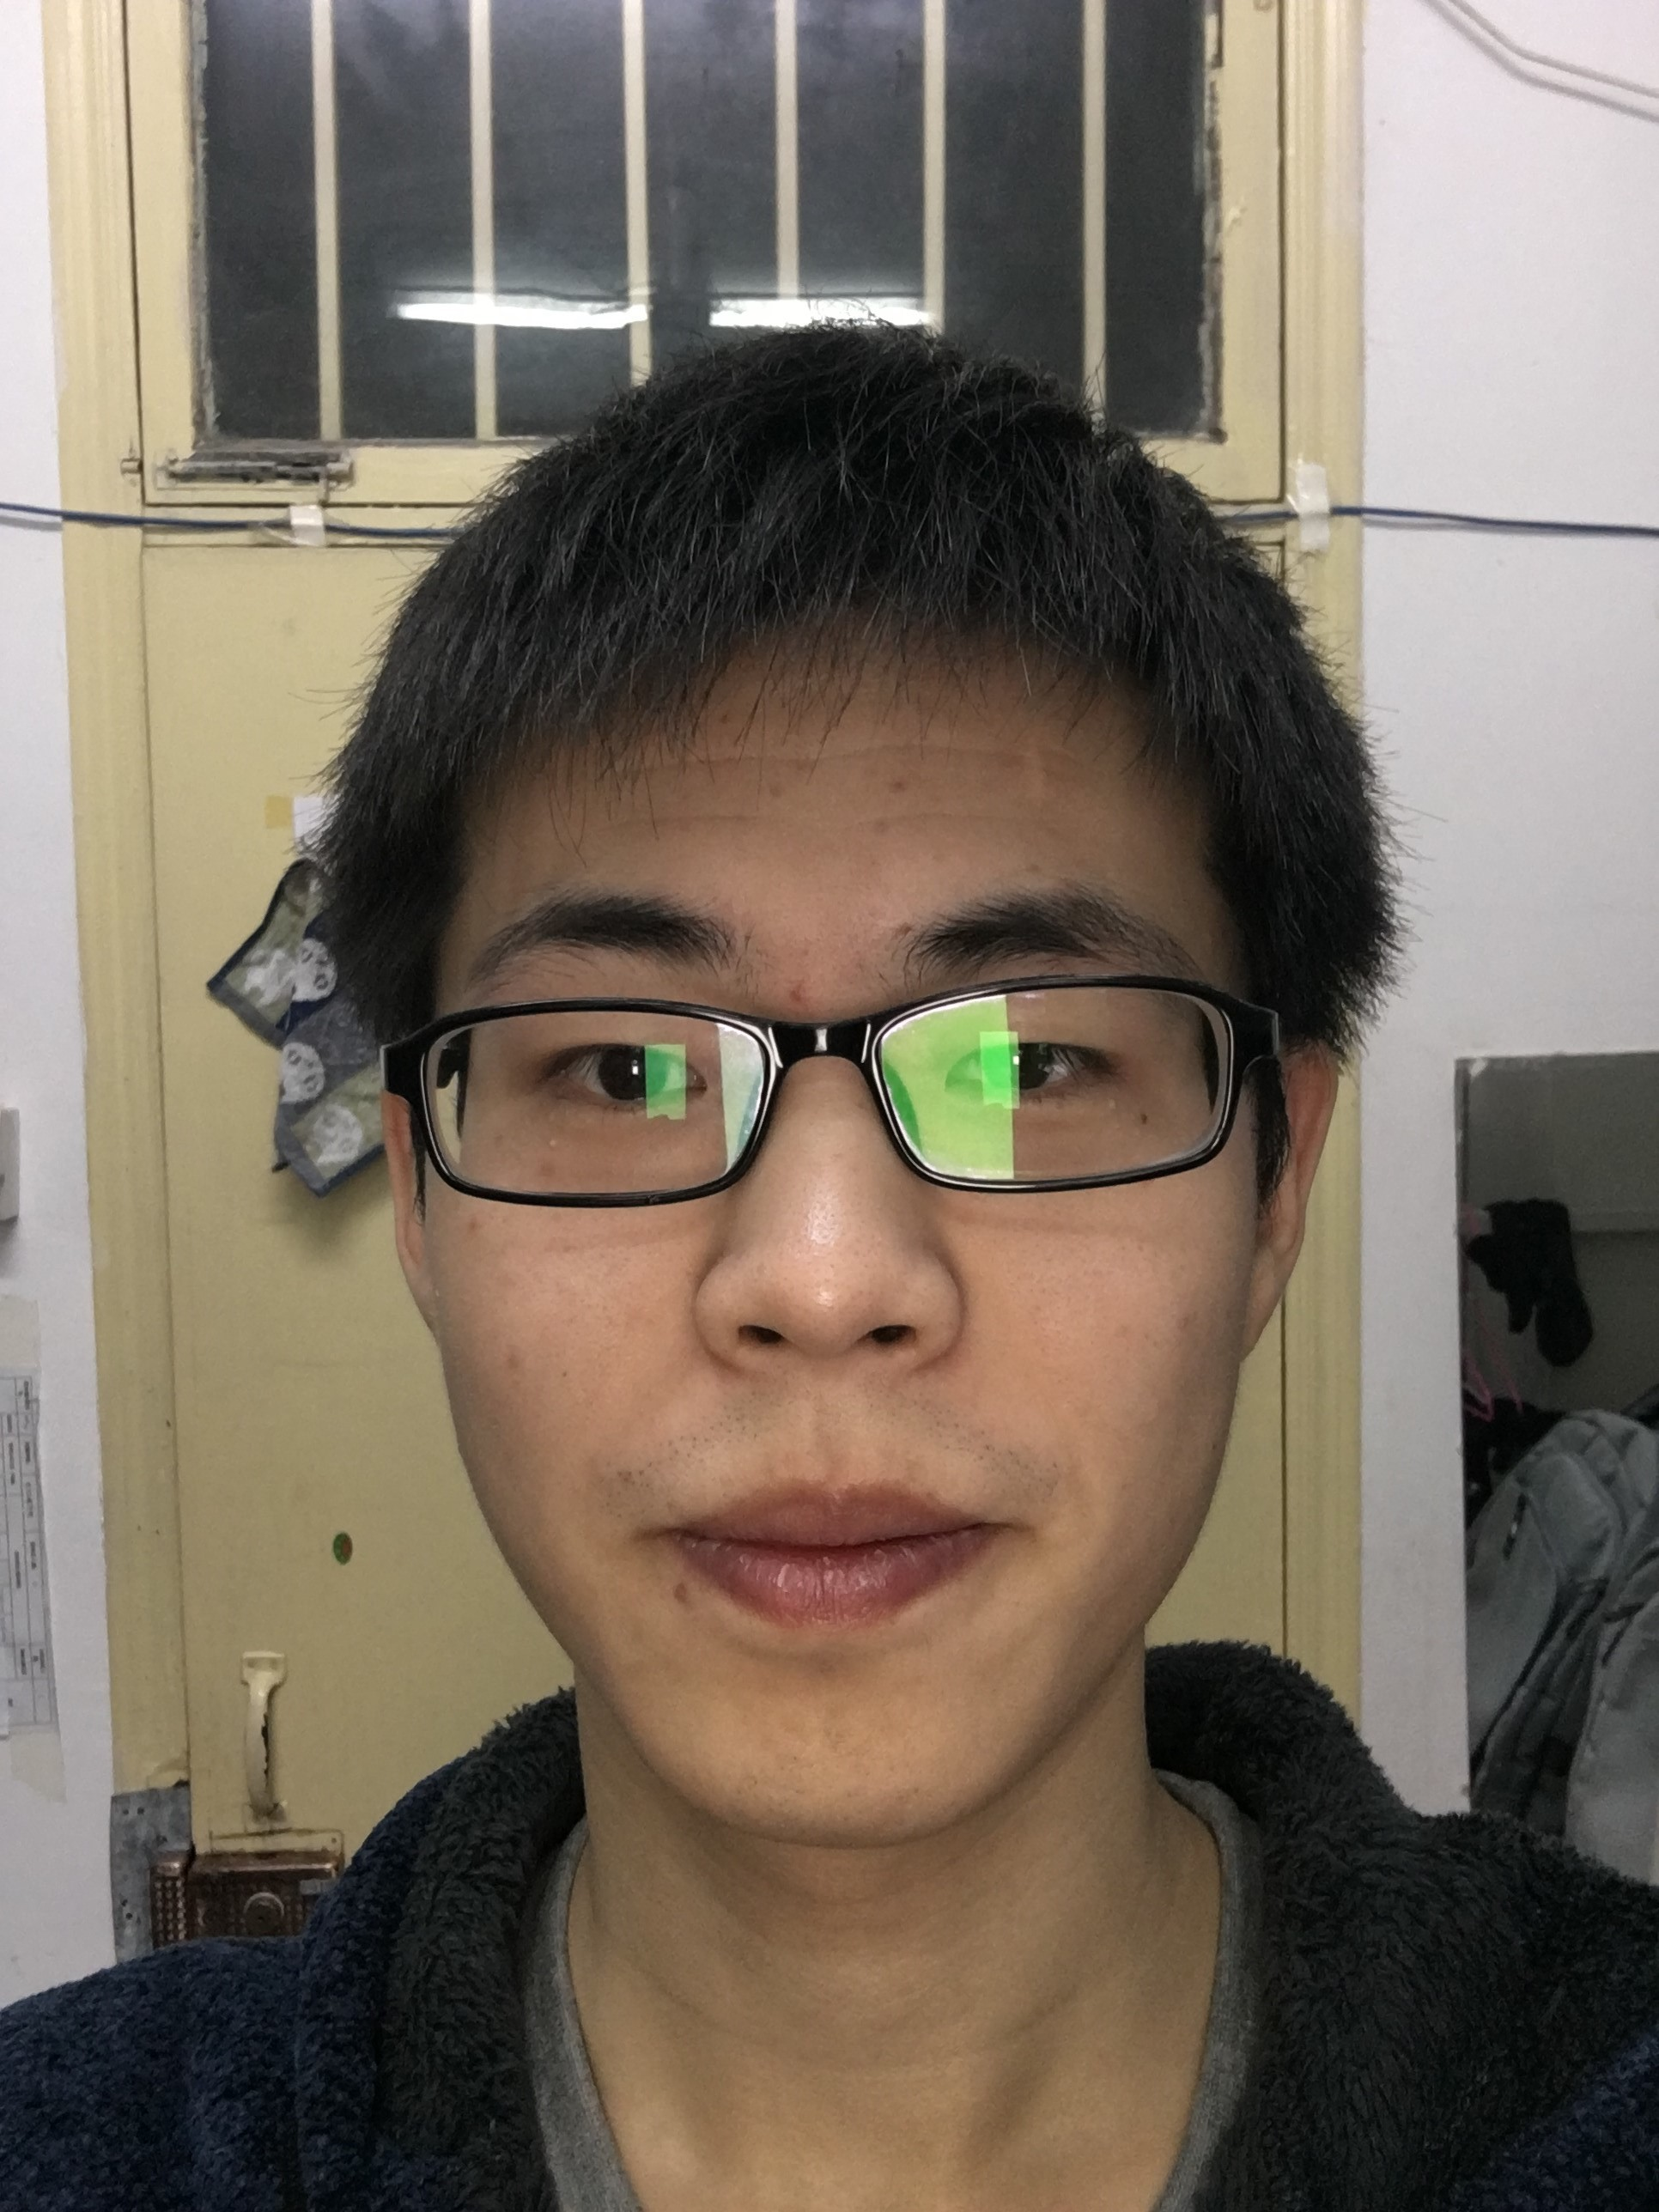
\includegraphics[width=18mm, height=24mm]{lishaogang.jpg} & 
\includegraphics[width=18mm, height=24mm]{Wangyuan.jpg} & 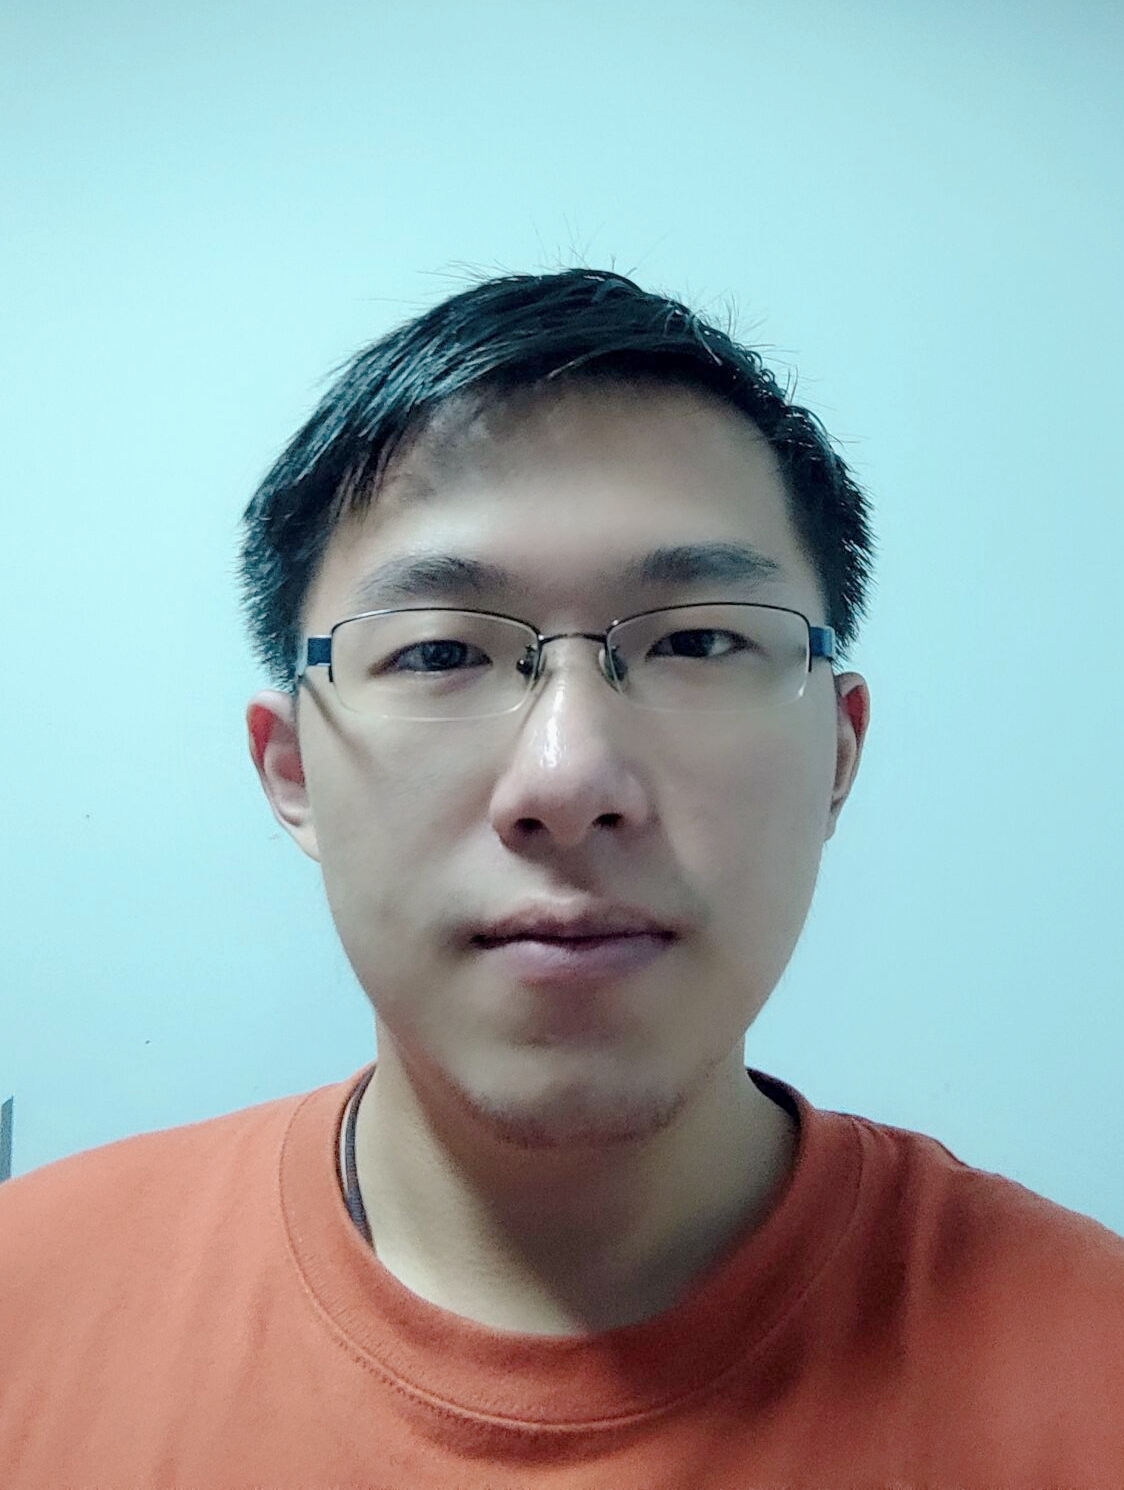
\includegraphics[width=18mm, height=24mm]{Ruanhengyu.jpg} & 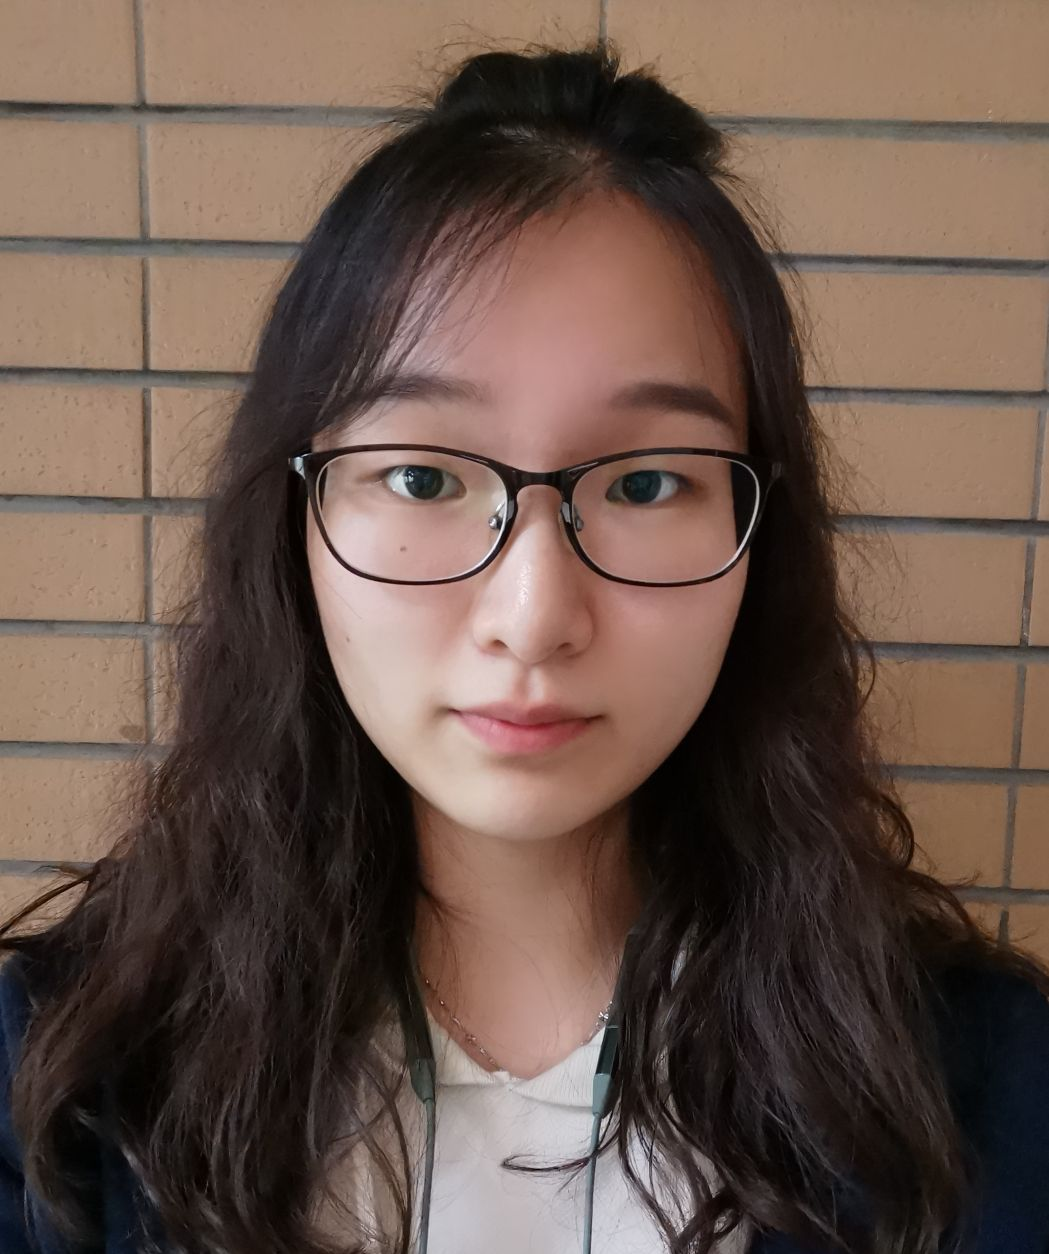
\includegraphics[width=18mm, height=24mm]{Aimee.jpg}\\\hline
				
				\color{blue}\textbf \textrm{Role} & Repository Manager & Data Manager & Bibliography Manager & Document Manager\\\hline
				
				\color{blue}\textbf \textrm{Accomplish Together} & \multicolumn{4}{c|}{Define roles , Improve question , Doodle question and Report}\\ \hline
			
			\end{tabular}  
		\end{center}  
	\end{table}  

	
	
	
	
\end{document}
